\documentclass{article}

\usepackage[a4paper]{geometry}
\usepackage{graphicx}
\usepackage{hyperref}
\usepackage{csquotes}
\usepackage[parfill]{parskip}
\usepackage{fancyhdr}
\usepackage{ragged2e}

\geometry{textwidth=15.75cm, textheight=23.4cm, marginratio={4:6,5:7}}
\graphicspath{ {./images/} }

\pagestyle{fancy}
\fancyhead[R]{Not for Distribution - Embargoed until 5/13/24}
\fancyhead[L]{tiksan [238332]}

\begin{document}
\begin{center}
	\begin{large}
		Torn Discord Account Linking Vulnerability Disclosure
	\end{large}
\end{center}

\raggedright

\par{\textbf{TL;DR:} Torn has a vulnerability in its process of linking Torn and Discord accounts allowing impersonation of Torn users on Discord servers and some third-party websites that support Discord-based login. Users should avoid clicking on links that go to \url{https://torn.com/discord.php} to avoid being impacted by this vulnerability.

\tableofcontents

\section{Introduction} \label{sec:introduction}
\par{In compliance with \href{https://www.torn.com/forums.php#/p=threads&f=1&t=16141356&b=0&a=0}{Torn's bug bounty policy} (see figure~\ref{fig:bug-bounty-policy} in the Appendix) and common Coordinated Vulnerability Disclosure policy, this is a public disclosure of an unresolved vulnerability in Torn's system to link Discord and Torn accounts together. This disclosure comes on the heels of a 30 day embargo/waiting period after first reporting the issue and a general lack of response from Torn staff and developers and a lack of willingness to fix this non-critical vulnerability (see figure \ref{fig:ched-response-1} in the Appendix). Torn uses a commonly used authorization specification known as OAuth2 to implement this feature to link Discord and Torn accounts. The data coming from this feature is commonly used in third-party, Torn-related tools and Discord bots (e.g. YATA, Tornium, Giving Tree, etc.) for account verification in Discord servers (see section \ref{sec:technical-details} for those of you who want more technical details). However, Torn's implementation of this features appears to meet the minimum requirements of the specification and the minimum shown by Discord's implementation of this feature in their quickstart/documentation \cite{discord-oauth-authorization-flow}. However, this means that Torn is missing a few of the highly recommended details mentioned in the specification(s) to prevent certain security issues. For example, this vulnerability would allow malicious users to send you a URL (such as \url{https://www.torn.com/discord.php?code=lUbv9hX241gEDWgc5igzxmGBKZT7yt}) that would be able to link their Discord account to your Torn account (making their Discord account to be shown as your Torn account after verification with one of various bots). This would work the other way around as well with a malicious user requesting the URL from you after Discord authentication to access your Discord account details (such as your email used for Discord, messages, etc.) provided a leak of a secret password-like value by Torn (the Discord application's client\_secret).}

\par{Previously, this vulnerability would have been worse. I can't find the bug report for this, but about a year ago (from what I remember) there was a separate (CSRF) vulnerability in this system that allowed account linking without any user input/interaction required. For example, all that's required would be an image on someone's profile that has the Discord linking URL as its source and a user could be automatically linked to someone else's account without their knowledge. This is why defense in depth is important as the recommended implementation details prevent attacks in case one security practice/implementation fails.}

\subsection{Is This Being Exploited?}
\par{There's no way for me to know if this is being actively exploited or has been in the past given the difficulty in collaborating with Torn developers/staff. But there have been previous instances of users being able to read messages and/or receiving push notifications for messages in servers (specifically faction leadership servers) they should not and are not in which could have been caused by this vulnerability. There have also been instances of users accidentally and non-maliciously linking their Discord account to other people's due to this vulnerability. This could indicate that this vulnerability has potentially been exploited in the past. However, once again, there's no way for me to check this.}

\subsection{How Does This Impact Me?}
\par{This shouldn't actively impact individuals unless they'd already clicked one of these links or had shared this link previously. Assuming Torn does not come out with a fix/patch for this vulnerability, primarily users shouldn't follow a link to \url{https://torn.com/discord.php} from a third party (especially if there's a code value included in the URL) and click the button to verify your Torn nickname. Instead to link your Torn account with your Discord account, you can visit the Discord link at the top navigation bar on Torn and follow the links Torn's George bot will send to you on Discord. Also, you shouldn't share the URL that Discord provides after you authenticate through them as this theoretically allows malicious users to view certain Discord-related account details while appearing to be Torn.}

\par{Server admins that rely upon verification bots, especially for faction leadership servers, may be impacted as this would allow malicious users to impersonate another user for the purposes of verification (especially if verification isn't checked continuously). And there's no easy way to verify the accuracy of verification.}

\par{This vulnerability if exploited could possibly be reflected to other tools such as \href{https://tornium.com}{Tornium} and \href{https://tornuhc.eu}{UHC} depending on how the tools are developed potentially resulting in leaked API keys, leaked private faction data (e.g. member stats, vault movement), etc. Once again, there's nothing for users to do, and for developers of these tools there's not much that can be done to prevent this other than disabling Discord-based authentication/authorization and/or preventing sensitive data such as API keys from being viewable.}

\subsection{Coordinated Disclosure Policy}
\par{Coordinated Vulnerability Disclosure (CVD) is the process of disclosing a software/hardware vulnerability to the responsible parties while giving them sufficient time to resolve the issue before publicly releasing information regarding the vulnerability. In this case, as seen in the section \ref{sec:timeline}, Torn staff weren't responding to mails and Chedburn felt that 
\begin{displayquote}
	there are ways we could shore it up and make it fully secure against every possibility, but this isn’t banking software, it’s just account-discord verification.
\end{displayquote}
And as Torn doesn't feel that it's important to fix this and as staff fail to respond to mails regarding this, this public advisory has been/will be published 30 days from original notification (April 13th). Torn doesn't state an explicit timeframe for public disclosure only to
\begin{displayquote}
	provide us a reasonable amount of time to resolve the issue before any disclosure to the public or a third-party [\ref{fig:bug-bounty-policy}]
\end{displayquote}
and neither Chedburn nor Bogie responded adequately to questions regarding this, so I've chosen a common CVD public disclosure timeframe of 30 days (many other companies and government agencies also state 45 days and 90 days for comparison).}

\section{Technical Details} \label{sec:technical-details}
\par{This section is more for developers and people interested in the specifics of this vulnerability... Torn's OAuth flow is started with George bot (or a server's administrators/management bots) sending the user a link to a Discord OAuth link for George bot/Torn:}

\justifying
\begin{displayquote}
	\url{https://discord.com/oauth2/authorize?client_id=441210177971159041&redirect_uri=https%3A%2F%2Fwww.torn.com%2Fdiscord.php&response_type=code&scope=identify}
\end{displayquote}

\raggedright
\par{This authorization link includes the required parameters such as client\_id, redirect\_uri, and scope. However, this link does not indicate any of the optional security features included in the base OAuth2 specification (RFC 6749) or any of the extensions of the specification (such as RFC 7636 for Proof of Key Exchange) to prevent a Cross-Site Request Forgery (CSRF) exploit are supported by Torn despite being implemented by Discord \cite{discord-oauth-csrf} and strongly recommended by the IETF (the organization that developed the OAuth2 specification).}

\begin{displayquote}
	While Discord does not require the use of the `state` parameter, we support it and highly recommends that you implement it for the security of your own application and data.
\end{displayquote}

\par{In fact, the OAuth2 specification and its extensions (as well as various comments made by their authors) state that some/any CSRF is required to be implemented by the client \cite{oauth-csrf} and \cite{oauth-redirect-flow-protection}:}
\begin{displayquote}
	The client MUST implement CSRF protection for its redirection URI. \\
	This is typically accomplished by requiring any request sent to the \\
	redirection URI endpoint to include a value that binds the request to \\ 
	the user-agent's authenticated state (e.g., a hash of the session \\
	cookie used to authenticate the user-agent).  The client SHOULD \\
	utilize the "state" request parameter to deliver this value to the \\
	authorization server when making an authorization request. \\
\end{displayquote}
\begin{displayquote}
	Clients MUST prevent Cross-Site Request Forgery (CSRF). In this \\
	context, CSRF refers to requests to the redirection endpoint that do \\
	not originate at the authorization server, but a malicious third \\
	party (see Section 4.4.1.8. of [RFC6819] for details). Clients that \\
	have ensured that the authorization server supports Proof Key for \\
	Code Exchange (PKCE, [RFC7636]) MAY rely on the CSRF protection \\
	provided by PKCE. In OpenID Connect flows, the nonce parameter \\
	provides CSRF protection. Otherwise, one-time use CSRF tokens carried \\
	in the state parameter that are securely bound to the user agent MUST \\
	be used for CSRF protection (see Section 4.7.1).
\end{displayquote}

\subsection{An Attack Vector}
\begin{enumerate}
	\item The malicious user starts the OAuth process by authenticating with Discord granting the Torn's Discord application consent to user data, but does not finish the authentication process on Torn retaining the validity of the authorization code.
	\item Somehow, another Torn user is convinced to access this page while logged into Torn and press the button to link accounts.
	\item Attacker's authorization code is exchanged for an access token. Using this access token, Torn retrieves the attacker's Discord ID and stores the ID under the Torn user.
	\item Attacker is now authorized to access certain third-party tools and Discord servers with automatic verification as the authorized user.
\end{enumerate}

\par{Theoretically this vulnerability could also be used to perform clickjacking by chaining together other vulnerabilities or if someone more knowledgeable than me looked at this. This could allow a user to unknowingly link their Torn account to the malcious user's Discord account.}

\par{Additionally, as stated in Section \ref{sec:introduction}, the previous CSRF vulnerability in the OAuth flow would allow malicious users to inject an image or button or some other element that links to the malicious user's Discord OAuth callback URL with a pre-defined authorization code. Upon user interaction with the element, the resulting GET request would already be authenticated and could theoretically automatically link a user to the malicious user's Discord ID without any feedback from the user as there wouldn't be have been any CSRF protection or user-required actions that would prevent this.}

\subsection{State Parameter}
\par{The state parameter is included in the base OAuth2 specification to provide a way to maintain state between the client (the Torn website/app) and the resource server (Torn's servers). This state can be and is intended to be used to prevent Cross Site Forgery Attacks upon the resource server as quoted below \cite{oauth-authorization-request}.}
\begin{displayquote}
	state \\
        RECOMMENDED.  An opaque value used by the client to maintain \\
        state between the request and callback.  The authorization \\
        server includes this value when redirecting the user-agent back \\
        to the client.  The parameter SHOULD be used for preventing \\
        cross-site request forgery as described in Section 10.12. \\
\end{displayquote}

\par{The state parameter when properly generated and stored by the client would prevent an invalid redirect and the aforementioned attack. The generated state value would be stored on the client before redirecting to the Discord OAuth page and sent with the authorization code after redirecting back to Torn. This would permit the client to validate the state paramter against the local copy to verify the request for OAuth and to open the authorization was triggered by itself.}

\subsection{Proof Key of Code Exchange}
\par{The Proof Key of Code Exchange specification (RFC 7636) extends the base OAuth2 specification to provide a method of verifying the authorization is done by the same client that is attempting to exchange the authorization code for the access token. This isn't as important for Torn as the client is confidential and Discord doesn't allow clients to make OAuth-related API calls without including the client secret, so this could mostly only prevent malicious browser extensions from intercepting authorization codes in addition to CSRF protection. You can find more regarding PKCE in the specification \cite{oauth-pkce}.}

\newpage
\section{Appendix}
\subsection{Timeline} \label{sec:timeline}
\par{Screenshots of messages regarding this to Torn staff can be found below.}

\begin{enumerate}
	\item 4/13/24 - Vulnerability discovered
	\item 4/13/24 - Original Report sent to CloudJumper
	\item 4/18/24 - Follow-up message sent to CloudJumper
	\item 4/18/24 - Forwarded original report to IceBlueFire
	\item 4/22/24 - Response received from Chedburn via IceBlueFire (see figure \ref{fig:ched-response-1})
	\item 4/23/24 - Additional details sent to Chedburn via IceBlueFire
	\item 5/04/24 - Follow-up sent to IceBlueFire
	\item 5/04/24 - Response received from IceBlueFire indicating that this won't be fixed
	\item 5/13/24 - Public disclosure published
\end{enumerate}

\subsection{Screenshots}
\par{Below you can find some screenshots of relevant information in Torn in the event that Torn changes the text. Better resolution version of these screenshots and additional screenshots of the full conversations can be found at \url{}.}

\begin{figure}[h!]
	\centering
	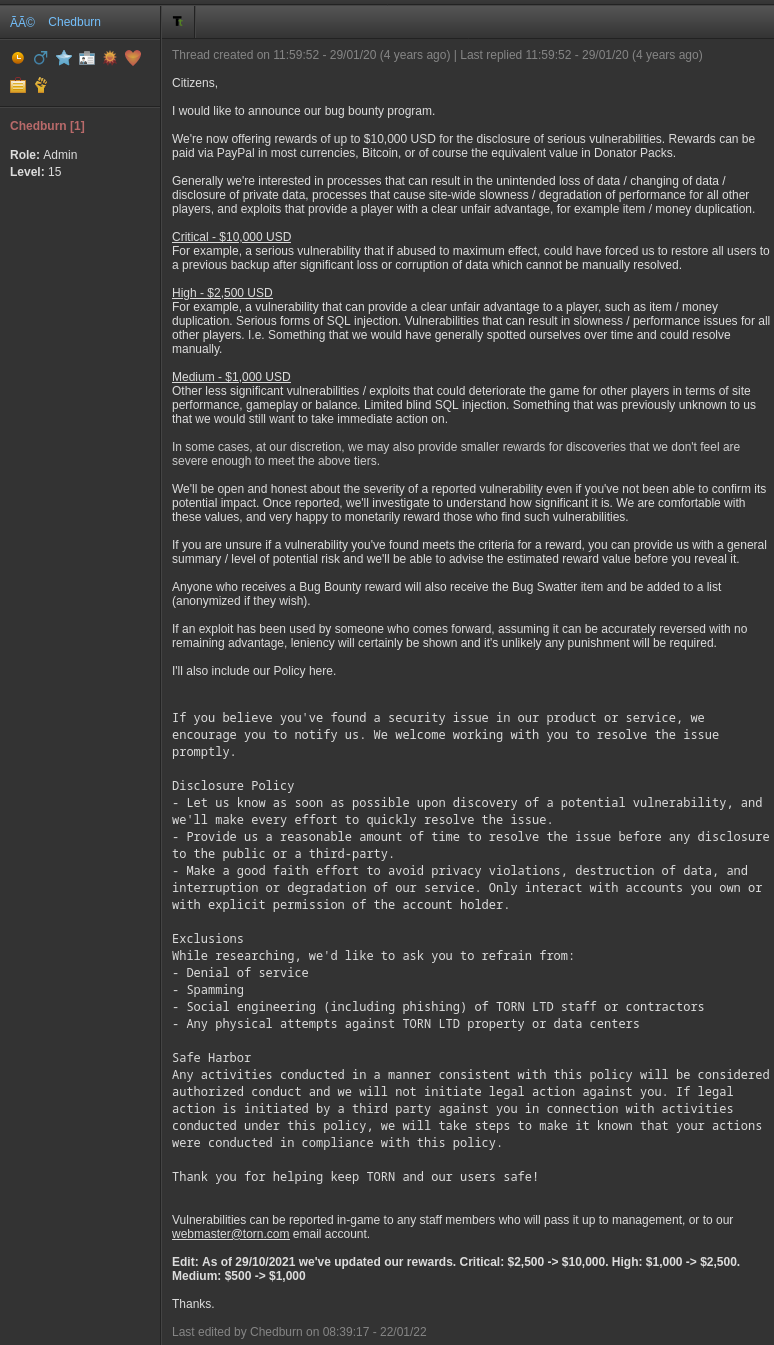
\includegraphics[scale=0.2]{torn-disclosure-policy.png}
	\caption{Torn's Bug Bounty policy}
	\label{fig:bug-bounty-policy}
\end{figure}

A current copy of the above screenshot can be found on \href{https://www.torn.com/forums.php#/p=threads&f=1&t=16141356&b=0&a=0}{Torn's forums}.

\begin{figure}[h!]
	\centering
	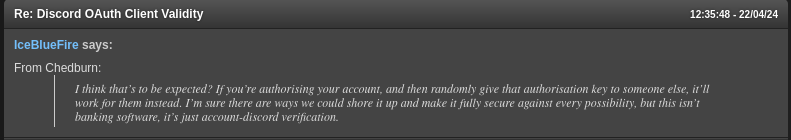
\includegraphics[scale=0.5]{ched-response-first.png}
	\caption{Ched's first response}
	\label{fig:ched-response-1}
\end{figure}

\newpage
\section{References}
\begin{thebibliography}{99}
	\bibitem{oauth-authorization-request} RFC6749: 4.1.1. Authorization Request \url{https://datatracker.ietf.org/doc/html/rfc6749#section-4.1.1}
	\bibitem{oauth-csrf} RFC6749: 10.12. Cross-Site Request Forgery \url{https://datatracker.ietf.org/doc/html/rfc6749#section-10.12}
	\bibitem{discord-oauth-csrf} Discord OAuth State and Security \url{https://discord.com/developers/docs/topics/oauth2#state-security}
	\bibitem{discord-oauth-authorization-flow} Discord OAuth Authorization Code Flow \url{https://discord.com/developers/docs/topics/oauth2#authorization-code-grant}
	\bibitem{oauth-redirect-flow-protection} IETF OAuth Security Topics Draft 27 \url{https://datatracker.ietf.org/doc/html/draft-ietf-oauth-security-topics-27#name-protecting-redirect-based-f}
	\bibitem{oauth-pkce} RFC7636: Proof Key for Code Exchange by OAuth Public Clients \url{https://datatracker.ietf.org/doc/html/rfc7636}
\end{thebibliography}

\end{document}
